\documentclass[12pt,a4paper]{article}
\usepackage{amsmath}
\usepackage{amsfonts}
\usepackage{amssymb}
\usepackage{graphicx}
\usepackage[left=2cm,right=2cm,top=2cm,bottom=2cm]{geometry}

\author{Gandham Phanikumar}
\title{A sample LaTeX document}

\date{June 07, 2022}

\begin{document}

\maketitle

\section{Introduction}

LaTeX allows one to think of typesetting in a structured manner - as opposed to visual manner. For programmers, this could be a natural way of putting down their thoughts.

\section{Discussion}

One of the important reasons why people choose LaTeX for document preparation is because of the way equations can be written and typeset.

\begin{equation}
	\text{erf}(\eta) = \frac{2}{\sqrt{\pi}} \int_{0}^{\eta}{ \text{exp}(-x^2) dx}
	\label{eqn:erf}
\end{equation}

You can refer to equations using their labels, for example eqn~\ref{eqn:erf} shows the definition of error function.

Bulleted items can be listed using the itemize environment.

\begin{itemize}
\item Each item starts with the item command.
\item You can nest them if you wish.
\end{itemize}

Numbered items can be listed using the enumerate environment.

\begin{enumerate}
\item There must be a formulation
\item It follows numerical implementation
\item Then comes the program development
\item Benchmarking is important
\item Original work can show up now
\end{enumerate}

Tables are formatted using the tabular environment. Each column is separated by an ampersand. The line ends with double backslash. Horizontal lines are given using the hline command. Vertical lines are given using pipe symbols in the options of tabular environment. The symbol l states that the column should be left justified. One can choose r or c for right or center justified columnds, respectively.

Tables can be referred to using their labels. For example, table~\ref{tab:progs} shows a list of linux programs and their utility.


\begin{table}
	\begin{center}
\begin{tabular}{|c|r|l|}
\hline
	& program & purpose \\
\hline
	1 & awk & Line by line processing - numerical and otherwise \\
	2 & sed & Line by line processing - string operations \\
	3 & python & Interpreted object oriented language \\
	4 & sage & Symbolic Computational environment \\
\hline
\end{tabular}
	\caption{Linux programs and their utility}
	\label{tab:progs}
	\end{center}
\end{table}

%--------------------------------------

\section{Image formats}

There are two major types of images.

\begin{enumerate}
	\item Raster images that contain pixel information. Popular formats are bmp, png, gif, jpg and tif.
	\item Vector images that contain object definitions and are rendered as per their size. Popular formats are eps, ps, pdf and svg.
\end{enumerate}

LaTeX can process eps files to include figures. If you need to insert other formats, use pdflatex. You can always convert images across formats using tools such as imagemagic on command line and gimp that works like Adobe Photoshop.

\section{Error function}

Here is a plot of error function.
 
\begin{figure}[h]
	\begin{center}
		\framebox{
			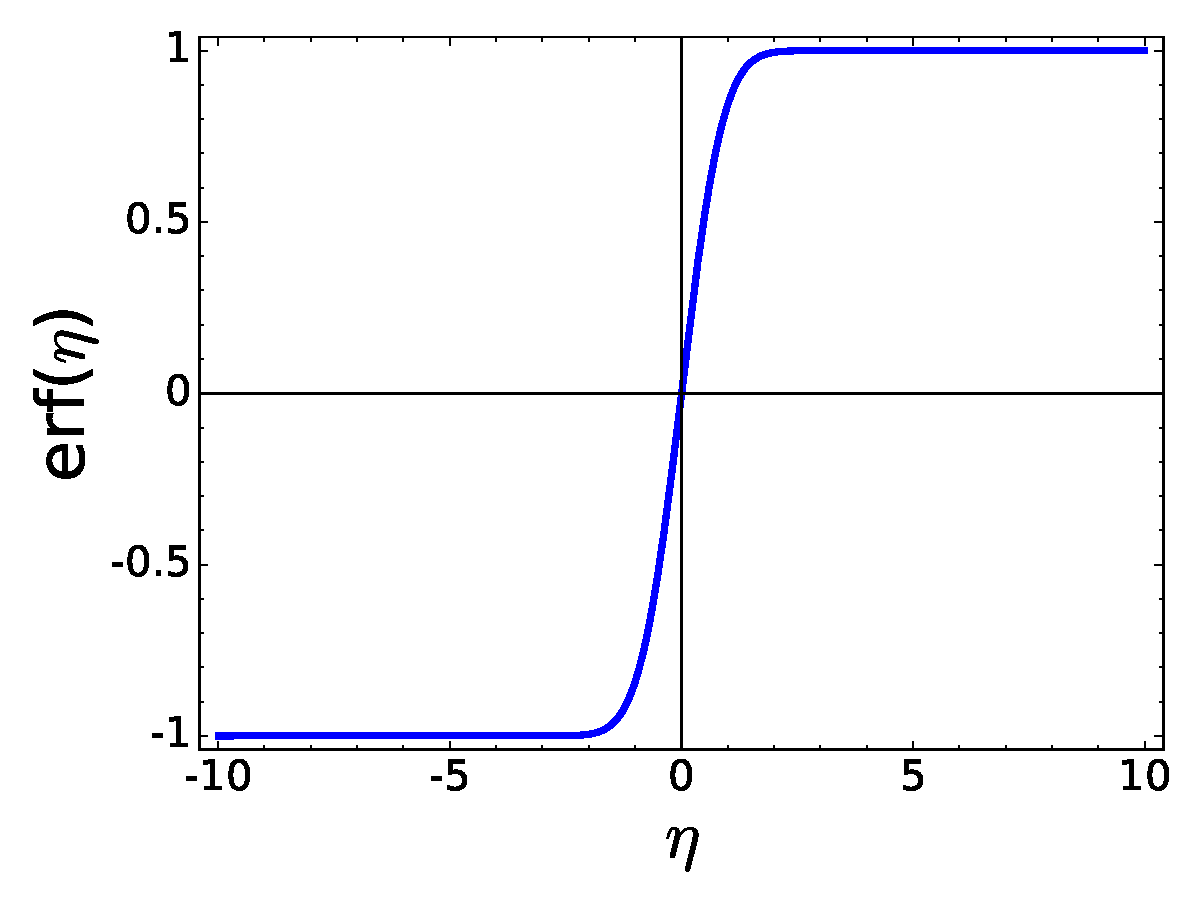
\includegraphics[scale=0.7]{erf.eps}
		}
	\end{center}
	\caption{A plot of error function made using sagemath.}
	\label{erfplot}
\end{figure}

You can refer to the figures using the ref command. For example, we can say we have shown the plot of error function in figure~\ref{erfplot}. Compile twice to ensure that the reference to the figure is available and typeset. The label command comes after the caption command inside the figure environment.

In this document we refer to two articles. The first is an article by Erian et al~\cite{erian}.  
The second is an article by Arie et al.~\cite{arie}. You must ensure the refs.bib file is in the same folder as this sample.tex file. After running latex you must run bibtex to have the references included. The recommended sequence of commands to make a final pdf is as follows:

\begin{enumerate}
	\item {\tt latex sample.tex} to compile tex file and create {\tt sample.dvi} file
	\item {\tt latex sample.tex} to ensure references for figures and equations
	\item {\tt bibtex sample} to look at {\tt sample.aux} to index and fetch bibliographic items as cited
	\item {\tt latex sample.tex} to include bibliographic references
	\item {\tt dvipdf sample.dvi} to create {\tt sample.pdf} 
\end{enumerate}

To make life easy, a Makefile has been provided along.

\section{Conclusion}

As you can see, document preparation can be like writing a program. Structured thinking can lead to neatly typeset documents with the help of LaTeX.

\bibliography{refs}
\bibliographystyle{alpha}

\end{document}
